\documentclass[aspectratio=169]{beamer}

\usepackage{ctex}
\usepackage{graphicx}
\usepackage{xcolor}

\usetheme{default}
\setbeamertemplate{navigation symbols}{}
\setbeamertemplate{footline}[frame number]

\definecolor{MTRRed}{RGB}{180, 32, 45}
\definecolor{DeepBlue}{RGB}{24, 60, 96}
\definecolor{SoftGray}{RGB}{245, 247, 250}
\definecolor{TextGray}{RGB}{64, 72, 80}

\setbeamercolor{title}{fg=DeepBlue}
\setbeamercolor{frametitle}{fg=DeepBlue}
\setbeamercolor{normal text}{fg=TextGray}
\setbeamercolor{block title}{fg=white,bg=DeepBlue}
\setbeamercolor{block body}{fg=TextGray,bg=SoftGray}
\setbeamertemplate{itemize item}{\color{MTRRed}\small$\blacktriangleright$}
\setbeamertemplate{itemize subitem}{\color{MTRRed}\scriptsize$\bullet$}
\graphicspath{{../screenshots/}}

\title{Part 2：交互界面与路线可解释性设计}
\subtitle{高胜寒完成部分}
\author{MTR Fare Optimizer \& Transit Interface}
\date{}

\begin{document}

\begin{frame}
  \titlepage
\end{frame}

\begin{frame}{我的负责范围：把算法结果变成可操作界面}
  \begin{columns}[T,onlytextwidth]
    \begin{column}{0.46\textwidth}
      \begin{block}{核心目标}
        \begin{itemize}
          \item 看得懂：路线、票价差异和地图位置同时可见
          \item 用得顺：桌面端和移动端都能完成规划任务
          \item 信得过：路线卡片与地图高亮互相印证
        \end{itemize}
      \end{block}
    \end{column}
    \begin{column}{0.50\textwidth}
      \begin{block}{本部分覆盖}
        \begin{itemize}
          \item 桌面端路线规划面板与地图联动
          \item 票价比较、节省金额和分段路线卡片
          \item 地图线路颜色、站点状态和图层开关
          \item 移动端地图优先布局与底部面板
        \end{itemize}
      \end{block}
    \end{column}
  \end{columns}

  \vspace{0.5em}
  \centering
  \color{DeepBlue}{\large 重点不是“美化界面”，而是降低认知负担并建立用户信任。}
\end{frame}

\begin{frame}{桌面端界面：路线规划与地图并列}
  \begin{columns}[T,onlytextwidth]
    \begin{column}{0.58\textwidth}
      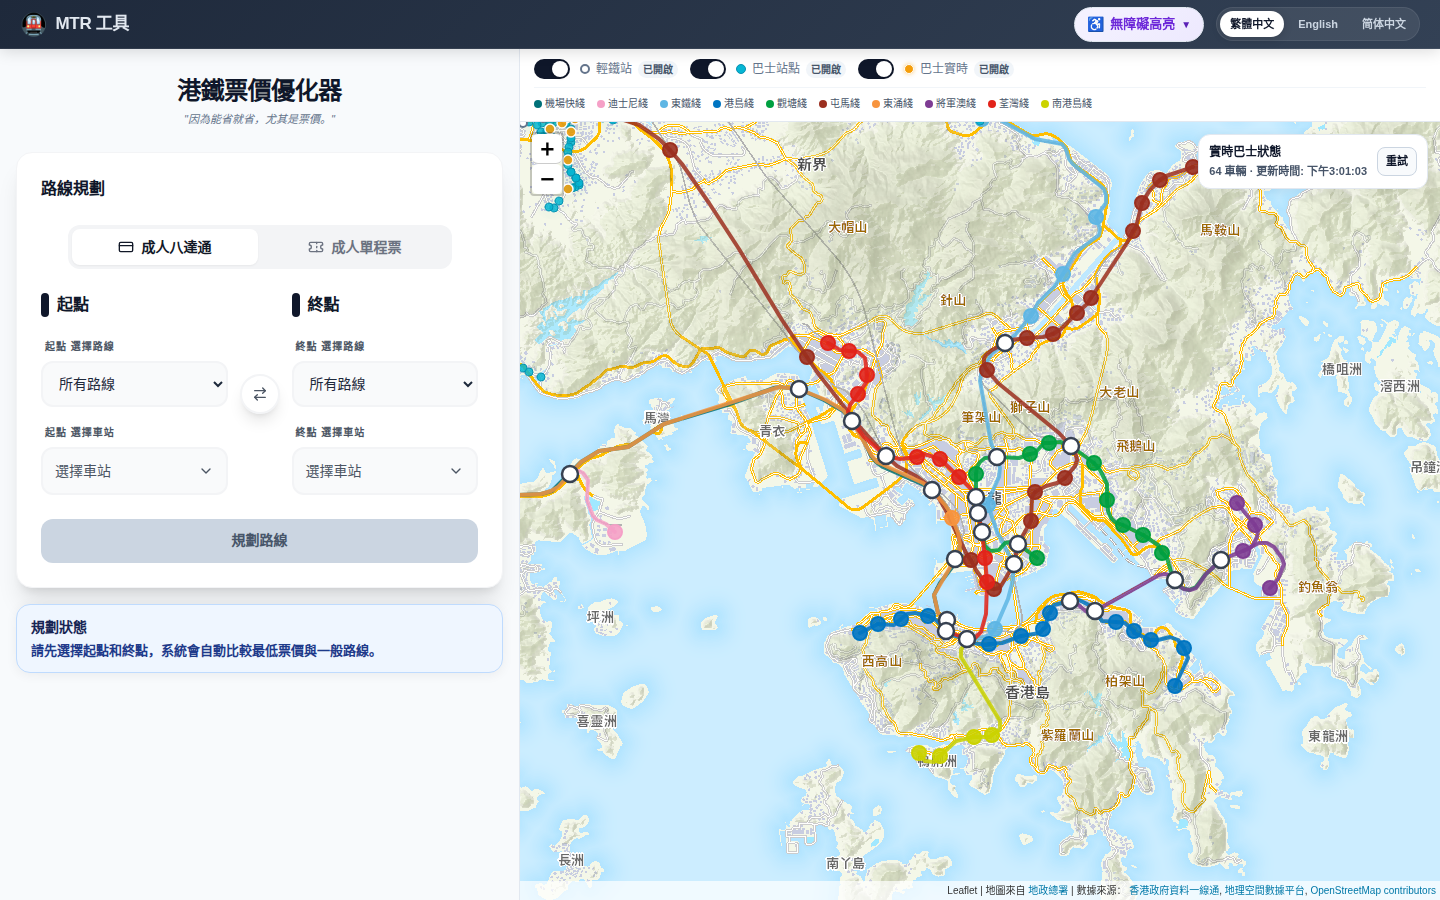
\includegraphics[width=\textwidth,height=0.70\textheight,keepaspectratio]{desktop-map-overview.png}
    \end{column}
    \begin{column}{0.38\textwidth}
      \begin{itemize}
        \item 左侧集中输入：票种、起点、终点和规划状态
        \item 右侧展示真实地图、线路、站点和交通图层
        \item 用户不用在表单页和地图页之间来回切换
        \item 对应 HCI 原则：可见性、空间映射、降低认知负荷
      \end{itemize}
    \end{column}
  \end{columns}
\end{frame}

\begin{frame}{路线结果展示：让用户看懂为什么省钱}
  \begin{columns}[T,onlytextwidth]
    \begin{column}{0.58\textwidth}
      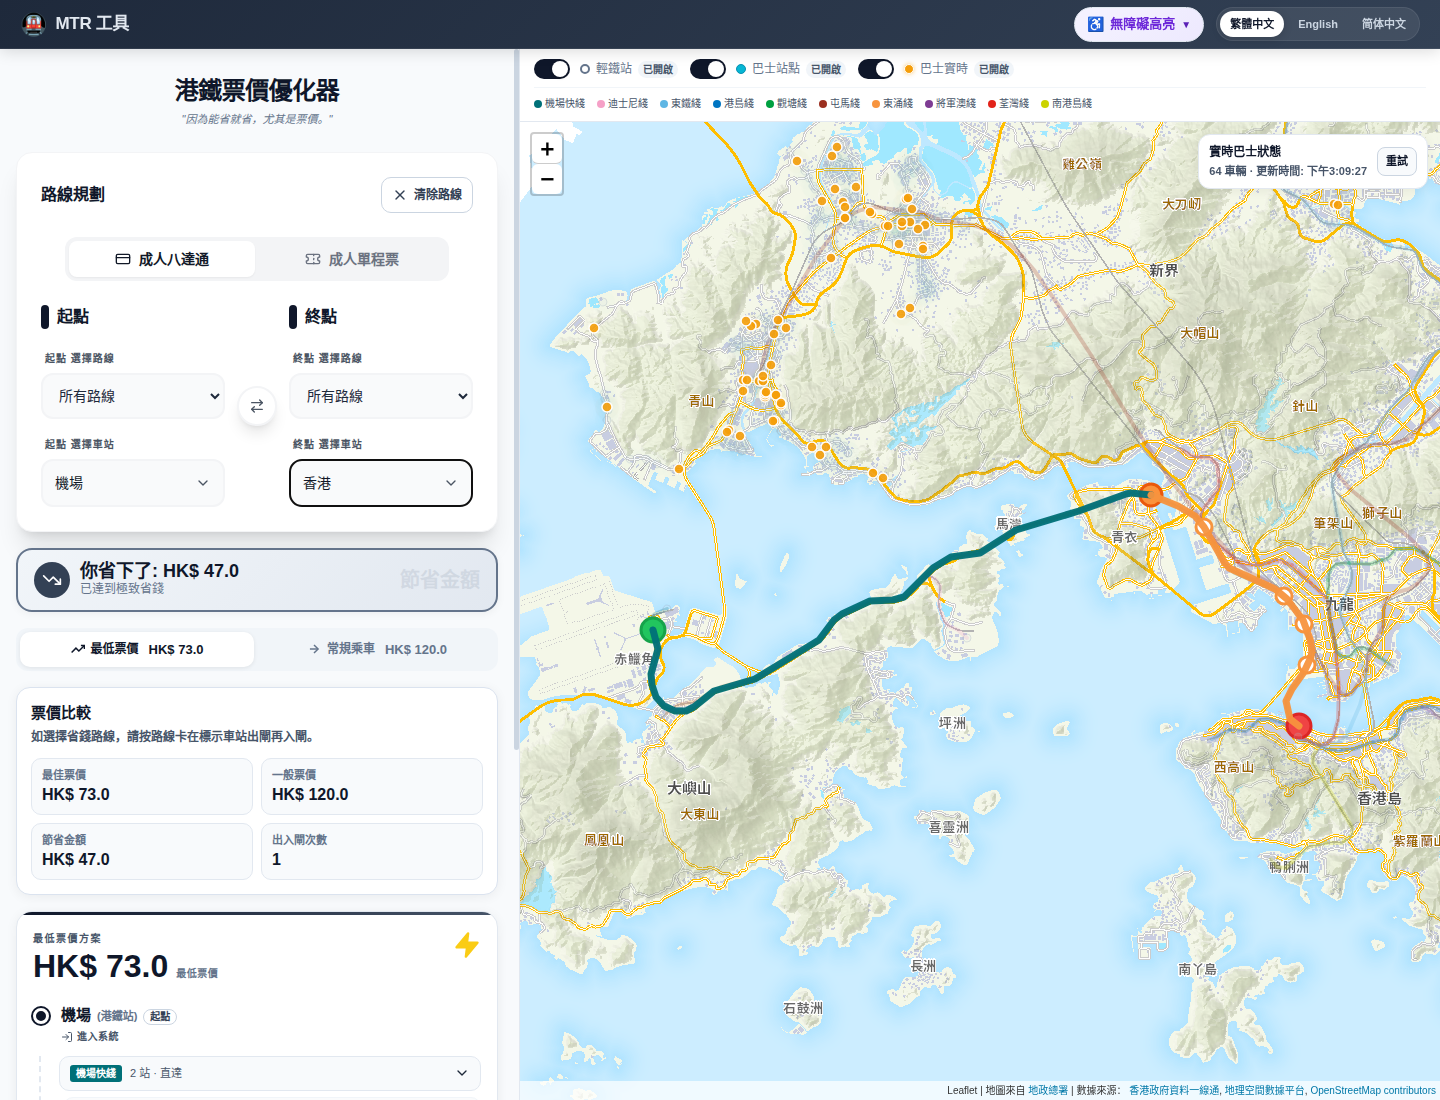
\includegraphics[width=\textwidth,height=0.72\textheight,keepaspectratio]{route-result-desktop.png}
    \end{column}
    \begin{column}{0.38\textwidth}
      \begin{block}{机场 $\rightarrow$ 香港案例}
        \begin{itemize}
          \item 最低票价：HK\$73.0
          \item 常规乘车：HK\$120.0
          \item 节省金额：HK\$47.0
        \end{itemize}
      \end{block}
      \begin{itemize}
        \item 用分段卡片说明线路、站点序列和出入闸行为
        \item 地图同步高亮路线，帮助用户验证推荐结果
        \item 对应 HCI 原则：反馈、可解释性、识别优于记忆
      \end{itemize}
    \end{column}
  \end{columns}
\end{frame}

\begin{frame}{地图线路显示：用视觉编码处理复杂网络}
  \begin{columns}[T,onlytextwidth]
    \begin{column}{0.42\textwidth}
      \begin{itemize}
        \item 真实底图与真实站点坐标提供空间参照
        \item 不同港铁线路使用稳定颜色，减少识别成本
        \item 起点、终点、当前路线和非当前站点形成视觉层级
        \item 轻铁站、巴士站、实时巴士通过图层开关控制信息密度
      \end{itemize}
    \end{column}
    \begin{column}{0.54\textwidth}
      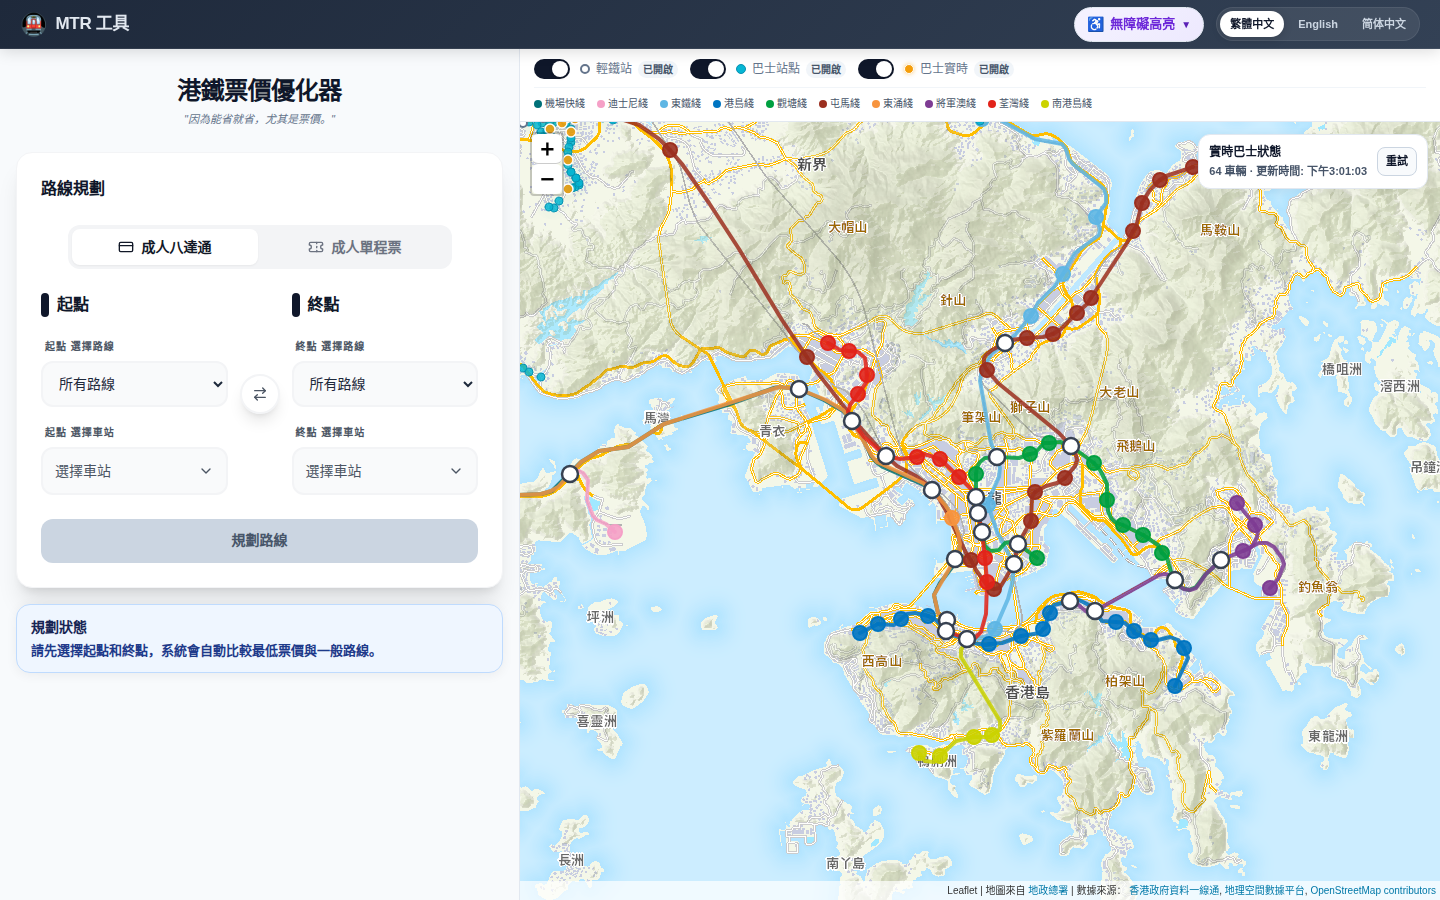
\includegraphics[width=\textwidth,height=0.72\textheight,keepaspectratio]{desktop-map-overview.png}
    \end{column}
  \end{columns}

  \vspace{0.25em}
  \centering
  \color{DeepBlue}{地图不是背景装饰，而是路线理解工具。}
\end{frame}

\begin{frame}{移动端适配：地图优先 + 底部面板}
  \begin{columns}[T,onlytextwidth]
    \begin{column}{0.30\textwidth}
      \centering
      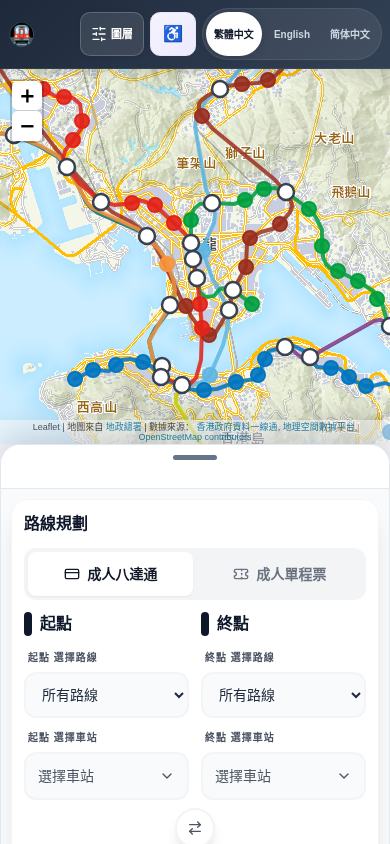
\includegraphics[width=0.88\textwidth,height=0.72\textheight,keepaspectratio]{mobile-overview.png}
    \end{column}
    \begin{column}{0.30\textwidth}
      \centering
      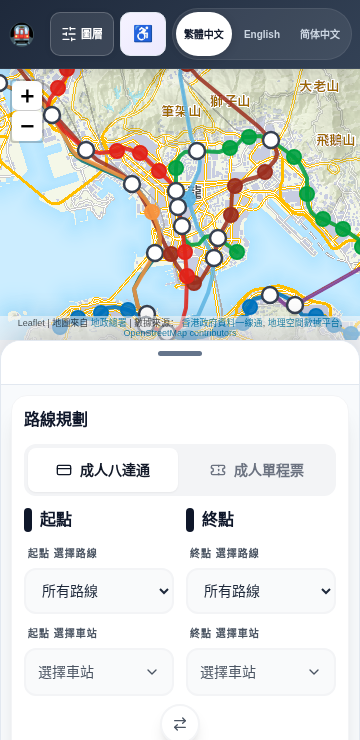
\includegraphics[width=0.82\textwidth,height=0.72\textheight,keepaspectratio]{mobile-narrow.png}
    \end{column}
    \begin{column}{0.36\textwidth}
      \begin{itemize}
        \item 移动端不是压缩桌面端，而是重新排序任务优先级
        \item 首屏保留地图，适配真实出行中的方向感需求
        \item 路线规划进入底部面板，支持展开、收起和拖拽
        \item 针对 390px、360px 窄屏处理遮挡和误触问题
      \end{itemize}
    \end{column}
  \end{columns}
\end{frame}

\begin{frame}{HCI 原则对应关系}
  \begin{columns}[T,onlytextwidth]
    \begin{column}{0.48\textwidth}
      \begin{block}{可见性与反馈}
        \begin{itemize}
          \item 规划状态、票价比较和节省金额即时显示
          \item 路线结果与地图高亮同步更新
        \end{itemize}
      \end{block}
      \begin{block}{用户控制}
        \begin{itemize}
          \item 图层开关控制信息密度
          \item 移动端底部面板由用户展开或收起
        \end{itemize}
      \end{block}
    \end{column}
    \begin{column}{0.48\textwidth}
      \begin{block}{识别优于记忆}
        \begin{itemize}
          \item 站点序列、线路标签、出入闸提示直接呈现
          \item 颜色和状态替代大段文字说明
        \end{itemize}
      \end{block}
      \begin{block}{情境适配}
        \begin{itemize}
          \item 桌面端强调并列对照
          \item 移动端强调地图优先和窄屏可用性
        \end{itemize}
      \end{block}
    \end{column}
  \end{columns}
\end{frame}

\begin{frame}{本部分小结}
  \begin{itemize}
    \item 桌面端通过“规划面板 + 地图”并列结构，把输入、反馈和空间位置放在同一任务空间。
    \item 路线结果通过票价比较、节省金额和分段卡片，让算法输出变成用户能执行的说明。
    \item 地图用线路颜色、站点状态、路线高亮和图层开关降低复杂网络的认知负担。
    \item 移动端采用地图优先和底部面板，贴合真实出行场景。
  \end{itemize}

  \vspace{0.8em}
  \centering
  \color{DeepBlue}{用界面结构降低认知负担，用视觉反馈建立用户信任。}
\end{frame}

\end{document}
